\chapter{From Rough Mix to Finished: A Full Song Walkthrough}
\label{chap:rough-to-finished}

\classquote{道虽迩，不行不至；事虽小，不为不成。}{《荀子·修身》 / Xunzi, "Self-Cultivation" (Xiu Shen)}{Translation: Though the road is near, without walking you do not arrive; though the task is small, without doing it you do not complete it. Note: rough mix to finished is a sequence of small, real actions.}

This chapter stops explaining devices one by one and walks a whole song from start to finish. The example is a 3:50 project with drums, bass, two guitars, lead vocal, backing vocals and strings, arranged as intro, verse 1, chorus 1, verse 2, chorus 2, bridge, final chorus and outro. The numbers below are experienced starting points, not built-in Yeban presets. Each step says what to change, how far to change it, and what has to be true before the step is done.

\begin{center}
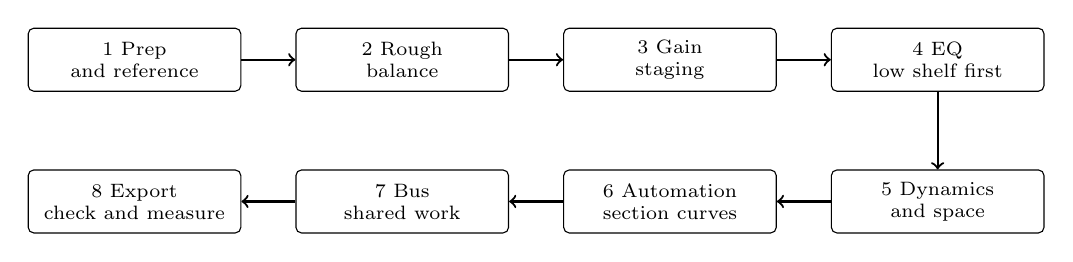
\begin{tikzpicture}[
  box/.style={draw, rounded corners=2pt, minimum width=27mm, minimum height=8mm, align=center, font=\scriptsize},
  arrow/.style={->, thick}
]
  \node[box] (prep) at (0,0) {1 Prep\\and reference};
  \node[box] (rough) at (3.4,0) {2 Rough\\balance};
  \node[box] (gain) at (6.8,0) {3 Gain\\staging};
  \node[box] (eq) at (10.2,0) {4 EQ\\low shelf first};
  \node[box] (dyn) at (10.2,-1.8) {5 Dynamics\\and space};
  \node[box] (auto) at (6.8,-1.8) {6 Automation\\section curves};
  \node[box] (bus) at (3.4,-1.8) {7 Bus\\shared work};
  \node[box] (out) at (0,-1.8) {8 Export\\check and measure};
  \draw[arrow] (prep) -- (rough);
  \draw[arrow] (rough) -- (gain);
  \draw[arrow] (gain) -- (eq);
  \draw[arrow] (eq) -- (dyn);
  \draw[arrow] (dyn) -- (auto);
  \draw[arrow] (auto) -- (bus);
  \draw[arrow] (bus) -- (out);
\end{tikzpicture}
\end{center}

The eight steps are not eight isolated buttons; they form a chain with a way back. If a step does not sound right, return to the previous step instead of forcing it on the master bus. The section table gives the checkpoints for the example; a real song may change the timings, but every section still needs one sentence saying what it should add or remove compared with the previous section.

\begin{table}[htbp]
\centering
\small
\begin{tabular}{@{}p{0.16\linewidth}p{0.15\linewidth}p{0.34\linewidth}p{0.27\linewidth}@{}}
\hline
Section & Time & Goal for this section & Main action \\
\hline
Intro & 0:00--0:35 & Establish pulse, keep headroom & Rough balance, no bus processing \\
Verse 1 & 0:35--1:10 & Vocal words clear; drums and bass do not fight & Faders, low shelf, vocal compression \\
Chorus 1 & 1:10--1:45 & One step up from the verse, not by forcing faders & Vocal automation, space, bus glue \\
Verse 2 & 1:45--2:20 & New texture, not a copy of verse 1 & Guitar delay or a different part, vocal dynamics \\
Chorus 2 & 2:20--2:55 & Bigger than chorus 1, more layers & Backing vocals, double, auxiliary return \\
Bridge & 2:55--3:15 & Drop down, expose the vocal & Drums step back, vocal up, shorter reverb \\
Final chorus & 3:15--3:35 & Loudest point, still not muddy & All tracks in, bus limiter catches peaks \\
Outro & 3:35--3:50 & Clean tail, no abrupt cut & Reverb tail, volume fade \\
\hline
\end{tabular}
\caption{Section goals for the example song}
\label{tab:walk-sections}
\end{table}

\section{Preparation and the reference track}

Save the project once, then check the sample rate in the audio settings. The export dialog defaults to \texttt{auto}, which follows the project; do not change the sample rate only at export time. For a reference track, use ``File $\rightarrow$ Import audio file...''. Yeban's GUI import accepts WAV, AIF and AIFF only; other formats have to go through the MCP import path. A file picker that ignores a FLAC is not a broken project.

After importing, select an audio track and use ``Track $\rightarrow$ Place the most recently imported audio on the current audio track''. There is no separate ``reference track'' type and no automatic loudness match: the reference is an ordinary audio track and it still goes through the master bus. For A/B, use solo/mute and bypass that track's devices. Do not claim a ``reference bus that bypasses the master''; Yeban has no such entry.

Use the reference to set direction, not numbers: listen to its low-end density, the place of the lead vocal in the mix, and how far the chorus lifts. Then return to your own project and make relative decisions. Do not copy the reference's LUFS as your target, and do not leave the reference track in the final export.

\section{Rough balance and gain staging}

Solo drums, bass and lead vocal first; mute everything else. Start the faders around $-12$ dB and keep the master at $0$ dB. Set the peak relationship among those three groups before adding guitars and strings. Do not push every fader to $0$ dB at the start: a fader position is not a ``correct answer'', only a level control.

\begin{table}[htbp]
\centering
\small
\begin{tabular}{@{}p{0.24\linewidth}p{0.22\linewidth}p{0.46\linewidth}@{}}
\hline
Control & Yeban range & Use \\
\hline
Track fader & $-60$ to $+6$ dB & Start rough balance at $-12$ dB; do not use it to repair clipping in the source \\
Pan & $-1$ to $+1$ & Default $0$; keep the rhythmic skeleton centred, offset guitars and backing vocals slightly \\
Send gain & $-60$ to $+12$ dB & Absolute dB; $0$ dB is unity, not ``percent'' \\
Master fader & $-60$ to $+6$ dB & Keep at $0$ while mixing; raising it feeds more level into the master inserts and export limiter \\
Track meter & Peak and RMS in dBFS & Starting points: kick about $-6$, bass about $-9$, lead vocal about $-6$, guitars about $-12$; not automatic targets \\
Master meter & Peak/RMS in dBFS; LUFS derived from RMS & Keep the master peak around $-6$ to $-3$ dBFS while mixing, leaving room for bus work \\
\hline
\end{tabular}
\caption{Controls and starting points for rough balance}
\label{tab:walk-controls}
\end{table}

Gain staging is not ``make every track equally loud''. The channel strip has separate input and output gain, both $-60$ to $+24$ dB; today neither has a GUI slider, so they are written through MCP or the project JSON. The visible fader is another level control. Pulling a fader down does not repair clipping in the source, and pushing it up does not give the device chain more headroom. Look at the track peak meter first, then decide whether to replace the source, change the channel-strip gain, or move the fader.

In a 24-bit project there is no need to push every track to $0$ dBFS. Let kick, bass and lead vocal peak roughly in the $-9$ to $-3$ dBFS region, and leave about $-6$ dB on the master before bus processing. Then EQ boosts, compressor makeup and reverb wet level are less likely to hit the ceiling immediately. These are starting points, not automatic normalization; Yeban does not decide ``loud enough'' for you.

The listening test for rough balance: in verse 1, every word of the lead vocal is intelligible without reading a lyric sheet; when kick and bass play together, the bass low end does not smear the kick's impact; when chorus 1 arrives, the whole mix clearly lifts one step but the master peak does not sit at $0$. If that fails, return to faders and pan before adding EQ.

\screenshot{walkthrough-console}{Mixer console with at least six tracks; faders, pan, track meters and the master meter in one view}

\section{EQ, dynamics and space}

The first EQ rule is ``cut before boost''. Yeban's EQ device has three bands: low shelf, mid peak and high shelf. The ranges are low-shelf gain $-18$ to $+18$ dB and low-shelf corner $20$ to $1000$ Hz; mid gain $-18$ to $+18$ dB, centre $200$ to $8000$ Hz and $Q$ $0.3$ to $6$; high-shelf gain $-18$ to $+18$ dB and corner $1000$ to $16000$ Hz. The defaults are all $0$ dB, with low shelf at $200$ Hz, mid at $1000$ Hz with $Q=0.9$, and high shelf at $4000$ Hz.

The GUI, however, exposes only one low-shelf gain slider. After inserting an EQ, the device rack lets you drag \texttt{eq\_low\_gain}; the low-shelf corner stays at the default $200$ Hz. Mid, high, frequency and $Q$ have no GUI controls and must be written through MCP or the project JSON. Do not read ``insert EQ'' as ``all four bands are adjustable in the GUI''; there are no four knobs and no frequency readout.

So the GUI-only EQ pass has to stay narrow: use $1$ to $3$ dB of low-shelf gain and judge whether the low end becomes clearer or just muddier. If the target is the $80$ to $120$ Hz bass low end, the GUI's $200$ Hz shelf is not the same move; either change \texttt{eq\_low\_freq} through MCP or accept that this GUI version cannot do it. For narrow problems such as harshness, sibilance or nasality, start with a $1$ to $2$ dB mid-peak cut and $Q=0.9$; do not use a broad low shelf to crush them.

\screenshot{walkthrough-eq-low}{Device rack EQ panel showing only the low-shelf gain slider; frequency and mid/high bands are not visible}

\begin{table}[htbp]
\centering
\small
\begin{tabular}{@{}p{0.12\linewidth}p{0.46\linewidth}p{0.15\linewidth}p{0.17\linewidth}@{}}
\hline
Device & Key parameters and ranges & Defaults & GUI reach \\
\hline
EQ & Low gain $-18$ to $+18$ dB, low corner $20$ to $1000$ Hz; mid gain $-18$ to $+18$ dB, centre $200$ to $8000$ Hz, $Q$ $0.3$ to $6$; high gain $-18$ to $+18$ dB, corner $1000$ to $16000$ Hz & All gains $0$; low $200$ Hz; mid $1000$ Hz, $Q=0.9$; high $4000$ Hz & Only low-shelf gain; frequency, mid and high go through MCP/JSON \\
Compressor & Threshold $-120$ to $+24$ dBFS, ratio $1$ to $1000$, knee $0$ to $24$ dB, detector $0.0001$ to $10$ s, attack $0.0001$ to $10$ s, release $0.0001$ to $10$ s, makeup $-24$ to $+24$ dB & Threshold $-12$, ratio $4$, knee $6$ dB, detector $5$ ms, attack $10$ ms, release $100$ ms, makeup $0$ & Track menu can insert; device rack only cycles ratio $2/4/8/20$; other parameters go through MCP/JSON \\
\hline
\end{tabular}
\caption{EQ and compressor parameter check}
\label{tab:walk-eq-comp}
\end{table}

The compressor's default is threshold $-12$ dBFS, ratio $4:1$, knee $6$ dB, detector $5$ ms, attack $10$ ms, release $100$ ms and makeup $0$ dB. The GUI can do only two things: insert one from the Track menu, or click the compressor row in the device rack to cycle the ratio through $2/4/8/20$. There are no threshold, attack, release or makeup sliders. The row reads ``Compressor: threshold ... ratio ... GR 0.0 dB'', but that $GR$ is a fixed string, not a live gain-reduction meter; do not use it to decide how much compression is happening. Set threshold and time constants through MCP; for listening, bypass A/B and judge whether transients survive and syllables stay clear.

The listening test for compression is not ``a bigger GR number is better''. After vocal compression, consonants are still clear, long notes do not pump, and the breath between phrases is not flattened. After bass compression, the low end does not pump but peaks no longer hit the master. After bus compression, the whole song glues together instead of every section being flattened to the same loudness. With no real GR meter, do not chase a number.

Space processing splits into insert and send. An insert reverb sits on a track and processes both dry and wet; a send reverb sits on an auxiliary return, and the source track only sends a copy of its signal there. Yeban's reverb defaults to Room type, \texttt{reverb\_size} $0.45$, \texttt{reverb\_damp} $0.35$, \texttt{reverb\_wet} $0.25$ and a $12$ ms pre-delay. \texttt{reverb\_wet} is the wet/dry mix: $0.25$ means about one quarter wet and three quarters dry.

That is the shared-reverb trap. Put a default \texttt{reverb\_wet} of $0.25$ on an auxiliary return and the return sends $75\%$ of the dry signal back into the master, on top of the source track's dry signal: double dry. A shared reverb needs \texttt{reverb\_wet} close to $1.0$ so the dry path is near $0$. That parameter has no GUI slider today and must go through MCP/JSON. The GUI's ``insert reverb'' is suitable for a track insert, not for a shared return at its default.

\screenshot{walkthrough-compressor}{Compressor row showing threshold, ratio and the GR string; the GR string is not a live meter}

\begin{table}[htbp]
\centering
\small
\begin{tabular}{@{}p{0.12\linewidth}p{0.50\linewidth}p{0.14\linewidth}p{0.16\linewidth}@{}}
\hline
Device & Key parameters and ranges & Defaults & GUI reach \\
\hline
Reverb & Size $0$ to $1$, kind $0$ to $3$ (Room/Plate/Hall/Spring), T60 $0$ to $10$ s, damping $0$ to $1$, wet mix $0$ to $1$, pre-delay $0$ to $0.1$ s & Room, size $0.45$, damping $0.35$, wet $0.25$, pre-delay $12$ ms & Insert and bypass; parameters go through MCP/JSON \\
Delay & Time $0.001$ to $2$ s, feedback $0$ to $0.95$, wet $0$ to $1$, damping $0$ to $1$, ping-pong $0/1$, sync $0/1$, numerator/denominator $1$ to $16$, dotted $0/1$ & Time $0.3$ s, feedback $0.3$, wet $0$, ping-pong $1$, sync off & No GUI entry to insert; if already in the project, bypass only; parameters through MCP/JSON \\
Limiter & Threshold $-30$ to $0$ dB, ceiling $-6$ to $0$ dB, release $10$ to $1000$ ms, lookahead $1$ to $192$ frames, true peak $0/1$ & Threshold $-1$, ceiling $-0.3$, release $80$ ms, lookahead $48$, true peak on & No GUI entry to insert; parameters through MCP/JSON \\
\hline
\end{tabular}
\caption{Space, delay and limiter parameter check}
\label{tab:walk-space-limiter}
\end{table}

Do not stack lead-vocal and guitar space on the same track: use a short reverb for the vocal and a delay for the guitar; if both are wet, the chorus turns to mush. For mono compatibility, press F4 to open the control room, switch MONO and listen for lost low end or backing vocals, then switch SIDE to hear only the difference. These switches change monitoring only, not the export. If bass or lead vocal collapses in MONO, return to pan and width instead of forcing a master EQ.

\section{Automation}

Automation should lock in differences between sections, not draw every beat. Yeban's automation targets are volume, pan, send gain, device parameters, macros and MIDI CC. Today the GUI can only click an existing lane to add or edit points; it cannot create or delete a lane, drag a point, change the curve, or switch read/write mode. When no lane exists, create it through MCP or the project JSON first; do not keep clicking an empty arrangement and expect a lane to appear.

The volume lane's nominal vertical axis is $-60$ to $+12$ dB, while the visible fader itself is $-60$ to $+6$ dB. These are not the same range. Use $+1$ to $+3$ dB for normal section lifts; do not write $+12$ into automation and then ask why the sound is wrong. Set the track's static fader near the target first, then check whether the automation points are absolute dB. Read is enabled by default; turn it off and playback and export fall back to the static value.

\begin{table}[htbp]
\centering
\small
\begin{tabular}{@{}p{0.21\linewidth}p{0.16\linewidth}p{0.17\linewidth}p{0.36\linewidth}@{}}
\hline
Target & Section & Value & Reason \\
\hline
Lead vocal volume & Chorus 1 & $+1.5$ dB & Lift the chorus without forcing the whole track fader \\
Lead vocal volume & Bridge & $-3$ dB & Pull back and expose guitar/strings \\
Lead vocal volume & Final chorus & $+2$ dB & Loudest point, still leaving master headroom \\
Guitar volume & Verse 2 & $-2$ dB & Change texture, do not fight verse 1 \\
Reverb send & Chorus 1 & $-6$ dB & Add tail without sending more dry signal \\
Reverb send & Bridge & $-12$ dB & Shorten the space and expose the vocal \\
\hline
\end{tabular}
\caption{Automation points for the example song}
\label{tab:walk-automation}
\end{table}

Write two to four points per section, at section boundaries and emotional turns; do not write a point every bar or the curve becomes noise. Points interpolate between each other with exact endpoints; clicking within $8$ pixels of an existing point edits it instead of creating a duplicate. The listening test is ``you cannot hear the automation moving'': the vocal should seem to grow naturally from verse to chorus, not like someone pulled a fader.

\screenshot{walkthrough-automation}{Arrangement view with a volume lane and section points; lead-vocal track and chorus boundary visible}

\section{Bus and export}

At the bus stage, separate the two legs: an auxiliary return handles shared processing for a group, and the master bus handles the final pass for the whole song. Create an auxiliary return with ``Track $\rightarrow$ + New auxiliary bus track'', then point the group's send edges at it. A send edge carries gain only, with no pre/post switch; do not assume another DAW's send-point convention.

The master bus GUI device rack offers only EQ and reverb buttons; there is no master compressor button. For bus glue, select an auxiliary return, insert a Compressor from the Track menu, and send the drum group or the whole group into it. The master EQ low-shelf slider also changes only the low-shelf gain; frequency and mid/high bands go through MCP. Keep the master fader at $0$ dB; raising it feeds more level into the inserts and export limiter, so do not use it to ``compensate'' the limiter.

There are two limiters at export time and they must be kept apart. The device-chain Limiter is an ordinary insert: threshold default $-1$ dBFS, ceiling $-0.3$ dBFS, release $80$ ms, lookahead $48$ frames, true-peak detection on. Today the GUI has no button to insert it, and its parameters go through MCP/JSON. The export dialog's ``bus limiter'' is a different fixed-parameter limiter: threshold $0.9$ (about $-0.92$ dBFS), ceiling $0.95$ (about $-0.45$ dBFS), lookahead $33$ frames, true-peak detection off. It is off by default, is a per-export boolean, is not written into the project, and does not enter the undo stack.

\begin{table}[htbp]
\centering
\small
\begin{tabular}{@{}p{0.18\linewidth}p{0.29\linewidth}p{0.45\linewidth}@{}}
\hline
Control & Default & Notes \\
\hline
Output path & Empty = host default & Type it or use ``Browse...''; filling the field does not export \\
Sample rate & \texttt{auto} & Follows the project; enter Hz only when you really need a change \\
Bit depth & \texttt{24} & 16/24 integers use TPDF dither; 32f float passes through without dither \\
Duration & Project audible end & Clearing it falls back to 8 seconds; it is not ``selected clip'' \\
Bus limiter & Off & This export only; fixed parameters, not loudness normalization \\
\hline
\end{tabular}
\caption{The real controls in the WAV export dialog}
\label{tab:walk-export-controls}
\end{table}

\screenshot{walkthrough-export}{WAV export dialog with the five controls and the post-export measurement line in one view}

After export the dialog writes ``Measured · true peak ... dBFS · integrated loudness ... LUFS · LRA ... LU''. All three values come from the same master measurement; if a value cannot be measured it says ``not measured'', and you must not read it as $0$. True peak uses $16\times$ oversampling, integrated loudness is gated, and LRA is the range of short-term loudness. They are not the control-room master meter's ``smoothed RMS minus $0.691$ dB'' LUFS. For a streaming target of $-14$ LUFS or EBU R128 $-23$ LUFS, the GUI has no loudness-target field; use the CLI/MCP path. Both presets carry a $-1$ dBTP ceiling, use a $0.5$ LU tolerance, and accept only $44.1/48/88.2/96$ kHz; other sample rates fail instead of silently falling back to $48$ kHz.

\section{Pre-export check}

Walk the list below before export. None of the steps requires listening to the whole song again, but each must have a reason it can pass.

\begin{table}[htbp]
\centering
\small
\begin{tabular}{@{}p{0.05\linewidth}p{0.25\linewidth}p{0.62\linewidth}@{}}
\hline
 & Check & Pass condition \\
\hline
1 & Project saved & Save once; export does not save the project for you \\
2 & Solo/mute & All solos off; the reference track and dead tracks are muted \\
3 & Master bus & Fader at $0$ dB; no unintended device left on in the insert chain \\
4 & Headroom & Master peak around $-6$ to $-3$ dBFS before export; not pinned at $0$ \\
5 & Format & Sample rate matches the project; 24-bit for delivery, 32f for intermediate \\
6 & Duration & Default is the project's audible end; clearing it gives 8 seconds, so do not clear it by accident \\
7 & Limiter & Use it only as a safety net; if on, remember it is fixed-parameter \\
8 & Measurement & Read true peak, integrated loudness and LRA; ``not measured'' is not 0 \\
\hline
\end{tabular}
\caption{Pre-export checklist}
\label{tab:walk-export-check}
\end{table}

If the export reports ``master clipped N samples, suggested trim X dB'', lower the master or the source by that suggestion and export again; do not force it down with the export limiter. The export limiter guarantees only its own ceiling region, not ``absolutely no clipping''. The $16\times$ true-peak meter still has inherent under-read. Leave about $1$ dB of margin for delivery and do not sit on $0$.

\section{Common misreadings and boundaries}

\begin{table}[htbp]
\centering
\small
\begin{tabular}{@{}p{0.34\linewidth}p{0.54\linewidth}@{}}
\hline
Common misreading & What is actually true \\
\hline
``The fader is gain staging'' & The fader is a level control; the channel strip has separate input/output gain, and a clipped source cannot be repaired by pulling the fader \\
``The master LUFS is the delivery integrated loudness'' & The master LUFS is smoothed RMS minus $0.691$ dB, not gated integrated loudness \\
``Compressor GR 0.0 dB means no compression'' & That GR is a fixed string, not a live gain-reduction meter; use bypass A/B \\
``Limiter row $-0.1$ dBTP is the real limiter'' & That row is a static placeholder and appears even without a limiter; do not treat it as a measurement \\
``EQ is one knob'' & The GUI exposes only low-shelf gain; frequency, mid and high go through MCP/JSON \\
``Insert reverb means size and wet are adjustable'' & The GUI inserts and bypasses only; parameters go through MCP/JSON \\
``The default shared reverb is fine'' & Default wet $0.25$ sends $75\%$ dry again, causing double dry; a shared return needs wet near $1.0$ \\
``Sends have pre/post'' & A send edge has gain only; there is no pre/post switch \\
``The GUI can create automation lanes'' & It can only click existing lanes; create/delete, drag points and curves go through MCP/JSON \\
``The export limiter is loudness normalization'' & It is a fixed-parameter safety net; loudness targets exist only in CLI/MCP \\
``True peak guarantees no clipping'' & $16\times$ true peak has inherent under-read; leave margin, do not treat it as a mathematical guarantee \\
\hline
\end{tabular}
\caption{Common misreadings in the rough-to-finished pass}
\label{tab:walk-pitfalls}
\end{table}

This table is also the boundary of the chapter: Yeban has no automatic mastering, automatic loudness matching, reference-track level alignment, send pre/post, dither-mode/noise-shaping choice, or one-button master compressor. Do not document a missing ability as ``coming later'', and do not map another DAW's entry onto Yeban. Chapter 9's bus order still holds: the master fader is before the insert chain, and the export limiter is after it. This chapter only adds the walkthrough, not a second signal path.

\section{Exercise}


\begin{exercise}
\begin{enumerate}
  \item Take an 8-bar song from rough mix to finished. Change one variable per step and write ``sensation--evidence--change--relisten'' in the project note.
  \item Do at least one ``export with limiter off for the baseline, then on'' comparison; do not judge loudness from control-room placeholder readings.
  \item Before delivery, listen under normal, DIM, MONO, and SIDE; record unresolved problems instead of silently skipping them.
\end{enumerate}
\end{exercise}

\section{Terms, screenshots and help mapping}

\begin{table}[htbp]
\centering
\small
\begin{tabular}{@{}p{0.21\linewidth}p{0.25\linewidth}p{0.21\linewidth}p{0.25\linewidth}@{}}
\hline
Chinese & English & Chinese & English \\
\hline
粗混 & rough mix & 静态平衡 & static balance \\
增益结构 & gain staging & 参考曲 & reference track \\
低架 & low shelf & 中频峰 & mid peak \\
高架 & high shelf & 软膝 & soft knee \\
检波窗口 & detector window & 补偿增益 & makeup gain \\
辅助返回 & auxiliary return & 发送边 & send edge \\
导出限制器 & export limiter & 门限积分响度 & gated integrated loudness \\
真峰值 & true peak & 响度范围 & loudness range (LRA) \\
抖动 & dither & 母线 & master bus \\
\hline
\end{tabular}
\caption{New terms in this chapter}
\label{tab:walk-terms}
\end{table}

\begin{table}[htbp]
\centering
\small
\begin{tabular}{@{}p{0.27\linewidth}p{0.36\linewidth}p{0.31\linewidth}@{}}
\hline
Shot name & UI state & Steps \\
\hline
\texttt{walkthrough-console} & Mixer console with at least six tracks; faders, pan, track meters and master meter in one view & Press X or F8, play verse 1, capture \\
\texttt{walkthrough-eq-low} & Device rack EQ panel showing only the low-shelf gain slider & Select lead vocal, insert EQ, drag low-shelf gain, capture \\
\texttt{walkthrough-\allowbreak compressor} & Compressor row showing threshold, ratio and the GR string & Insert Compressor from Track menu, click the row to cycle ratio, capture \\
\texttt{walkthrough-\allowbreak automation} & Arrangement volume lane with section points; lead vocal and chorus boundary visible & Press A, click the lane to add or edit points, capture \\
\texttt{walkthrough-export} & WAV export dialog with five controls and the post-export measurement line & File menu, export WAV, export once, capture \\
\hline
\end{tabular}
\caption{Screenshot list for this chapter}
\label{tab:walk-screens}
\end{table}

\begin{table}[htbp]
\centering
\small
\begin{tabular}{@{}p{0.34\linewidth}p{0.52\linewidth}@{}}
\hline
Section & In-app help anchor \\
\hline
Preparation and reference & \texttt{walkthrough-prep} \\
Rough balance and gain staging & \texttt{walkthrough-balance-gain} \\
EQ, dynamics and space & \texttt{walkthrough-processing} \\
Automation & \texttt{walkthrough-\allowbreak automation} \\
Bus and export & \texttt{walkthrough-bus-export} \\
Pre-export check & \texttt{walkthrough-export-check} \\
Common misreadings and boundaries & \texttt{walkthrough-boundaries} \\
\hline
\end{tabular}
\caption{Help-topic map for chapter 10}
\label{tab:walk-help}
\end{table}

\section*{Further Reading}
\begin{itemize}[leftmargin=1.5em]
\item \url{https://www.soundonsound.com/techniques} — Sound On Sound techniques: fill in section checks, bus checks, and delivery checks across a complete mix workflow.
\item \url{https://github.com/gradetwo/yeban} — Yeban repository: check the README and source for the real entries of export, measured rows, and the master-bus limiter.
\end{itemize}
